\documentclass[12pt, a4paper]{article}
\usepackage[utf8]{inputenc}
\usepackage[spanish]{babel}
\usepackage{graphicx}
\usepackage{booktabs}
\usepackage{geometry}
\usepackage[hidelinks]{hyperref}
\usepackage{natbib}
\usepackage{amsmath}
\usepackage{array}
\usepackage{float}
\usepackage{url}

\geometry{top=2.5cm, bottom=2.5cm, left=2.5cm, right=2.5cm}

\begin{document}

% --- CARATULA ---
\begin{titlepage}
    \centering
    \vspace*{1cm}

    {\Large \textbf{Universidad Andres Bello}}\\[0.5cm]
    {\large Facultad de Ingenieria}\\[0.2cm]
    {\large Ingenieria Civil Informatica}\\[2cm]

    {\Huge \textbf{Estudio Comparativo Avanzado de Arquitecturas CNN y Vision Transformers en Ultrasonido de Mama}}\\[1.5cm]

    {\Large Proyecto de Machine Learning: Vision Artificial}\\[2cm]

    \begin{flushright}
        \textbf{Integrantes:}\\
        Cristobal Flores Villegas\\
        Francisco Morales Diaz\\
        Matias Munoz Parraguirre\\
        Benjamin Pena Diaz\\[1cm]
        \textbf{Profesor:}\\
        Billy Mark Peralta Marquez\\[1cm]
        \textbf{Fecha:}\\
        7 de Junio de 2026
    \end{flushright}
    \vfill
\end{titlepage}

\newpage
\tableofcontents
\newpage

% --- RESUMEN ---
\begin{abstract}
Este informe tecnico detalla el desarrollo y evaluacion de sistemas avanzados de aprendizaje de maquinas aplicados al dataset BreastMNIST, un benchmark de clasificacion binaria de imagenes de ultrasonido de mama. Se contrasta el rendimiento de arquitecturas convolucionales clasicas (MobileNetV2 y EfficientNetB0) frente a un Vision Transformer (ViT) personalizado, analizando el impacto de la resolucion espacial de entrada ($28\times28$ vs. $128\times128$ pixeles). Los resultados evidencian que las CNN ligeras con sesgos inductivos espaciales dominan sobre los Transformers en regimenes de datos pequenos, y que el desbalance de clases convierte al AUC-ROC en la metrica central del analisis, relegando a la exactitud a un rol meramente descriptivo.
\end{abstract}

% --- SECCION 1: INTRODUCCION ---
\section{Introduccion y Contexto Clinico}

El cancer de mama es la neoplasia mas frecuente en mujeres a nivel mundial y una de las principales causas de mortalidad oncologica femenina. La deteccion temprana es el factor pronostico mas determinante: la tasa de supervivencia a cinco anos supera el 90\% en estadios iniciales, mientras que en estadios avanzados desciende de forma drastica. La imagenologia juega un rol central en el tamizaje y diagnostico definitivo.

El ultrasonido mamario es una herramienta de primera linea, especialmente valiosa para mujeres con tejido mamario denso donde la mamografia convencional presenta sensibilidad reducida. Sin embargo, la interpretacion de imagenes ecograficas requiere expertise clinico considerable y es susceptible a variabilidad inter-observador significativa. En este contexto, los sistemas de diagnostico asistido por computador (\textit{Computer-Aided Diagnosis}, CAD) basados en aprendizaje profundo representan una solucion prometedora para estandarizar y escalar el proceso diagnostico.

El dataset BreastMNIST \citep{yang2023medmnist} estandariza este problema como una clasificacion binaria: imagenes de ultrasonido etiquetadas como malignas (clase 0) o benignas/normales (clase 1), preprocesadas a resolucion $28\times28$ pixeles. Este benchmark presenta dos desafios entrelazados: (1) la baja resolucion espacial, que limita la informacion disponible para las capas de extraccion de caracteristicas, y (2) un desbalance de clases inherente al dominio clinico, donde los casos benignos superan a los malignos reflejando la prevalencia real de la enfermedad.

Este trabajo investiga sistematicamente como distintas familias de arquitecturas de aprendizaje profundo se comportan bajo este regimen de datos limitado y baja resolucion. El objetivo es identificar que sesgos inductivos resultan mas beneficiosos para el diagnostico asistido y comprender las limitaciones fundamentales de cada enfoque desde una perspectiva teorica y empirica.

% --- SECCION 2: REVISION DE LITERATURA ---
\section{Revision de Literatura}

El aprendizaje profundo aplicado a imagenes medicas ha experimentado una evolucion acelerada desde la consolidacion de las redes convolucionales profundas. A continuacion se analizan tres trabajos indexados relevantes para este estudio, todos posteriores al anio 2018.

\subsection{MedMNIST v2: Benchmark Estandarizado para Imagenes Biomedicas}

\citet{yang2023medmnist} presentaron MedMNIST v2, una coleccion de 12 conjuntos de datos preprocesados de imagenes biomedicas 2D y 6 tridimensionales, disenada para democratizar la investigacion en vision artificial medica. La contribucion central reside en establecer un benchmark unificado con divisiones fijas de entrenamiento, validacion y prueba, eliminando la heterogeneidad metodologica que dificultaba la comparacion entre trabajos. Los autores evaluaron 10 modelos de referencia ---incluyendo ResNet-18, ResNet-50 y variantes de AutoML--- y reportaron que el AUC-ROC es la metrica mas informativa para datasets desbalanceados como BreastMNIST. Asimismo, documentaron que el accuracy simple colapsa hacia la clase mayoritaria, lo que constituye un hallazgo directamente aplicable a la interpretacion de nuestros resultados. Segun los autores, el BreastMNIST posee una distribucion de clases con aproximadamente 73\% de muestras benignas, lo que explica el techo de accuracy observado experimentalmente.

\subsection{Vision Transformer: Atencion Global para Reconocimiento Visual}

\citet{dosovitskiy2021vit} propusieron la arquitectura \textit{Vision Transformer} (ViT), demostrando que los mecanismos de auto-atencion pueden reemplazar las capas convolucionales en tareas de reconocimiento visual a gran escala. La arquitectura divide la imagen en parches fijos, los proyecta a un espacio de embeddings y aplica bloques de atencion multi-cabeza (\textit{Multi-Head Self-Attention}) seguidos de capas \textit{feed-forward} con conexiones residuales. El trabajo establece una conclusion fundamental para este estudio: los ViT requieren pre-entrenamiento en datasets de gran escala (JFT-300M o ImageNet-21k, con cientos de millones de muestras) para superar a las CNN en conjuntos de datos convencionales. Con volumenes de datos insuficientes, los Transformers convergen peor que arquitecturas como ResNet, precisamente porque carecen del sesgo inductivo de localidad espacial y equivarianza a traslaciones que las convoluciones imponen de forma implicita. Esta limitacion teorica se verifico empiricamente en nuestros experimentos con BreastMNIST.

\subsection{Dataset BUSI: Ultrasonido de Mama Anotado}

\citet{aldhabyani2020busi} publicaron el dataset BUSI (\textit{Breast Ultrasound Images}), recopilando 780 imagenes de ultrasonido de mama con sus mascaras de segmentacion, clasificadas en tres categorias: normal, benigno y maligno. Los autores documentan con detalle los desafios especificos del ultrasonido como modalidad de imagen medica: ruido de speckle, variabilidad en el contraste entre tejidos, artefactos de shadowing acustico y alta dependencia del operador. Ademas, evidencian el desbalance de clases inherente al dominio clinico, donde los casos benignos superan en numero a los malignos, reflejando la prevalencia real de la patologia. Este trabajo contextualiza directamente los obstaculos encontrados en BreastMNIST: la distribucion de clases es identica en naturaleza, y las caracteristicas visuales de las imagenes de ultrasonido (bajo contraste, ruido intrinseco) explican por que la extraccion de caracteristicas discriminativas es un problema abierto que requiere arquitecturas cuidadosamente adaptadas.

% --- SECCION 3: METODOLOGIA ---
\section{Metodologia}

\subsection{Dataset y Distribucion de Clases}

El dataset BreastMNIST proviene de la plataforma MedMNIST v2 \citep{yang2023medmnist} y contiene imagenes de ultrasonido de mama en escala de grises. La Tabla~\ref{tab:distribucion} resume la distribucion de muestras y clases.

\begin{table}[H]
\centering
\caption{Distribucion del dataset BreastMNIST por split y clase}
\label{tab:distribucion}
\begin{tabular}{lccc}
\toprule
\textbf{Split} & \textbf{Total} & \textbf{Clase 0 (Maligno)} & \textbf{Clase 1 (Benigno/Normal)} \\
\midrule
Entrenamiento & 546  & $\approx$147 (27\%) & $\approx$399 (73\%) \\
Validacion    & 78   & $\approx$21 (27\%)  & $\approx$57 (73\%)  \\
Prueba        & 156  & 42 (27\%)           & 114 (73\%)          \\
\bottomrule
\end{tabular}
\end{table}

La proporcion de la clase mayoritaria (benigno/normal) en el conjunto de prueba es del 73.08\%, valor que coincide exactamente con el accuracy reportado por todos los modelos, siendo la signatura de colapso hacia la clase mayoritaria.

\subsection{Diseno Experimental y Pipelines de Datos}

Se utilizo la division hold-out fija provista por MedMNIST, garantizando reproducibilidad y comparabilidad con la literatura. Se implementaron dos pipelines diferenciados:

\textbf{Pipeline $28\times28$ (Fase 1 y Fase 2):} Normalizacion de valores de pixel al rango $[0,1]$ y replicacion del canal de escala de grises a tres canales RGB para compatibilidad con arquitecturas pre-entrenadas en ImageNet.

\textbf{Pipeline $128\times128$ (Fase 2):} Misma normalizacion y replicacion de canales, mas reescalado bilineal de $28\times28$ a $128\times128$ pixeles, evaluando si la expansion artificial de resolucion beneficia a arquitecturas disenadas para entradas de mayor dimension.

\subsection{Regularizacion y Data Augmentation}

Para mitigar el sobreajuste sobre el dataset limitado (546 muestras de entrenamiento) se aplicaron las siguientes tecnicas durante el entrenamiento:

\begin{itemize}
    \item \textbf{Volteo horizontal y vertical aleatorio} (\texttt{RandomFlip}): incrementa la variabilidad sin introducir distorsion semantica en ultrasonido.
    \item \textbf{Rotacion aleatoria} de hasta 15$^\circ$ (\texttt{RandomRotation}): simula variaciones en la posicion del transductor.
    \item \textbf{Zoom aleatorio} de hasta 10\% (\texttt{RandomZoom}): modela ligeras variaciones en la profundidad de escaneo.
    \item \textbf{Early Stopping}: monitoreo de \texttt{val\_loss} con paciencia de 4 epocas y restauracion de los mejores pesos, previniendo sobreajuste y reduciendo tiempo de computo.
\end{itemize}

\subsection{Arquitecturas Implementadas}

Se evaluaron cuatro configuraciones experimentales mediante \textit{Transfer Learning} y ajuste fino:

\textbf{MobileNetV2 --- Baseline ($28\times28$):} Arquitectura ligera con bloques de convolucion separable en profundidad, pre-entrenada en ImageNet. Elegida como baseline por su eficiencia computacional demostrada en dispositivos con recursos limitados. Las capas base se congelaron inicialmente y se agrego una cabeza de clasificacion binaria con activacion sigmoide. Opera sobre la resolucion nativa del dataset, sin interpolacion.

\textbf{EfficientNetB0 --- $128\times128$:} Red convolucional con escalado compuesto (\textit{compound scaling}), optimizada para maximizar el rendimiento bajo restricciones de parametros. Evaluada sobre imagenes reescaladas a $128\times128$ para aprovechar su diseno optimizado para resoluciones superiores. Se aplico fine-tuning sobre las ultimas capas convolucionales tras el calentamiento inicial.

\textbf{Vision Transformer Personalizado --- $28\times28$ y $128\times128$:} Se implemento un ViT desde cero, adaptando matematicamente el calculo de dimensiones de parches a ambos tamanos de entrada. Las implementaciones estandar de ViT asumen resoluciones minimas de $224\times224$; para $28\times28$ y $128\times128$, las capas \texttt{PatchExtract} y \texttt{PatchEmbedding} requirieron calculo manual de dimensiones de tensor. La arquitectura incluye bloques de Transformer con atencion multi-cabeza, normalizacion por capas (\textit{LayerNorm}) y conexiones residuales.

\subsection{Metricas de Evaluacion}

\begin{itemize}
    \item \textbf{AUC-ROC} (metrica principal): capacidad discriminativa del modelo independiente del umbral.
    \item \textbf{Accuracy}: exactitud global, interpretada con cautela ante el desbalance.
    \item \textbf{Recall (Sensibilidad)}: tasa de verdaderos positivos; critico para no omitir casos malignos.
    \item \textbf{Tiempo de entrenamiento}: relevante para viabilidad computacional en entornos clinicos.
\end{itemize}

% --- SECCION 4: RESULTADOS Y ANALISIS CRITICO ---
\section{Resultados y Analisis Critico Cruzado}

\subsection{Tabla Comparativa de Resultados}

\begin{table}[H]
\centering
\caption{Comparativa de modelos evaluados en el conjunto de prueba de BreastMNIST}
\label{tab:resultados}
\begin{tabular}{lcccc}
\toprule
\textbf{Modelo / Resolucion} & \textbf{Accuracy} & \textbf{AUC} & \textbf{Recall} & \textbf{Tiempo (min)} \\
\midrule
MobileNetV2 --- $28\times28$ (Baseline) & 0.7308 & \textbf{0.7214} & 1.0 & 0.27 \\
EfficientNetB0 --- $128\times128$       & 0.7308 & 0.6629          & 1.0 & 0.39 \\
ViT Personalizado --- $28\times28$      & 0.7308 & 0.4980          & 1.0 & 0.25 \\
ViT Personalizado --- $128\times128$    & 0.7308 & 0.5512          & 1.0 & 0.61 \\
\bottomrule
\end{tabular}
\end{table}

\subsection{Visualizacion: Matriz de Confusion}

\begin{figure}[H]
\centering
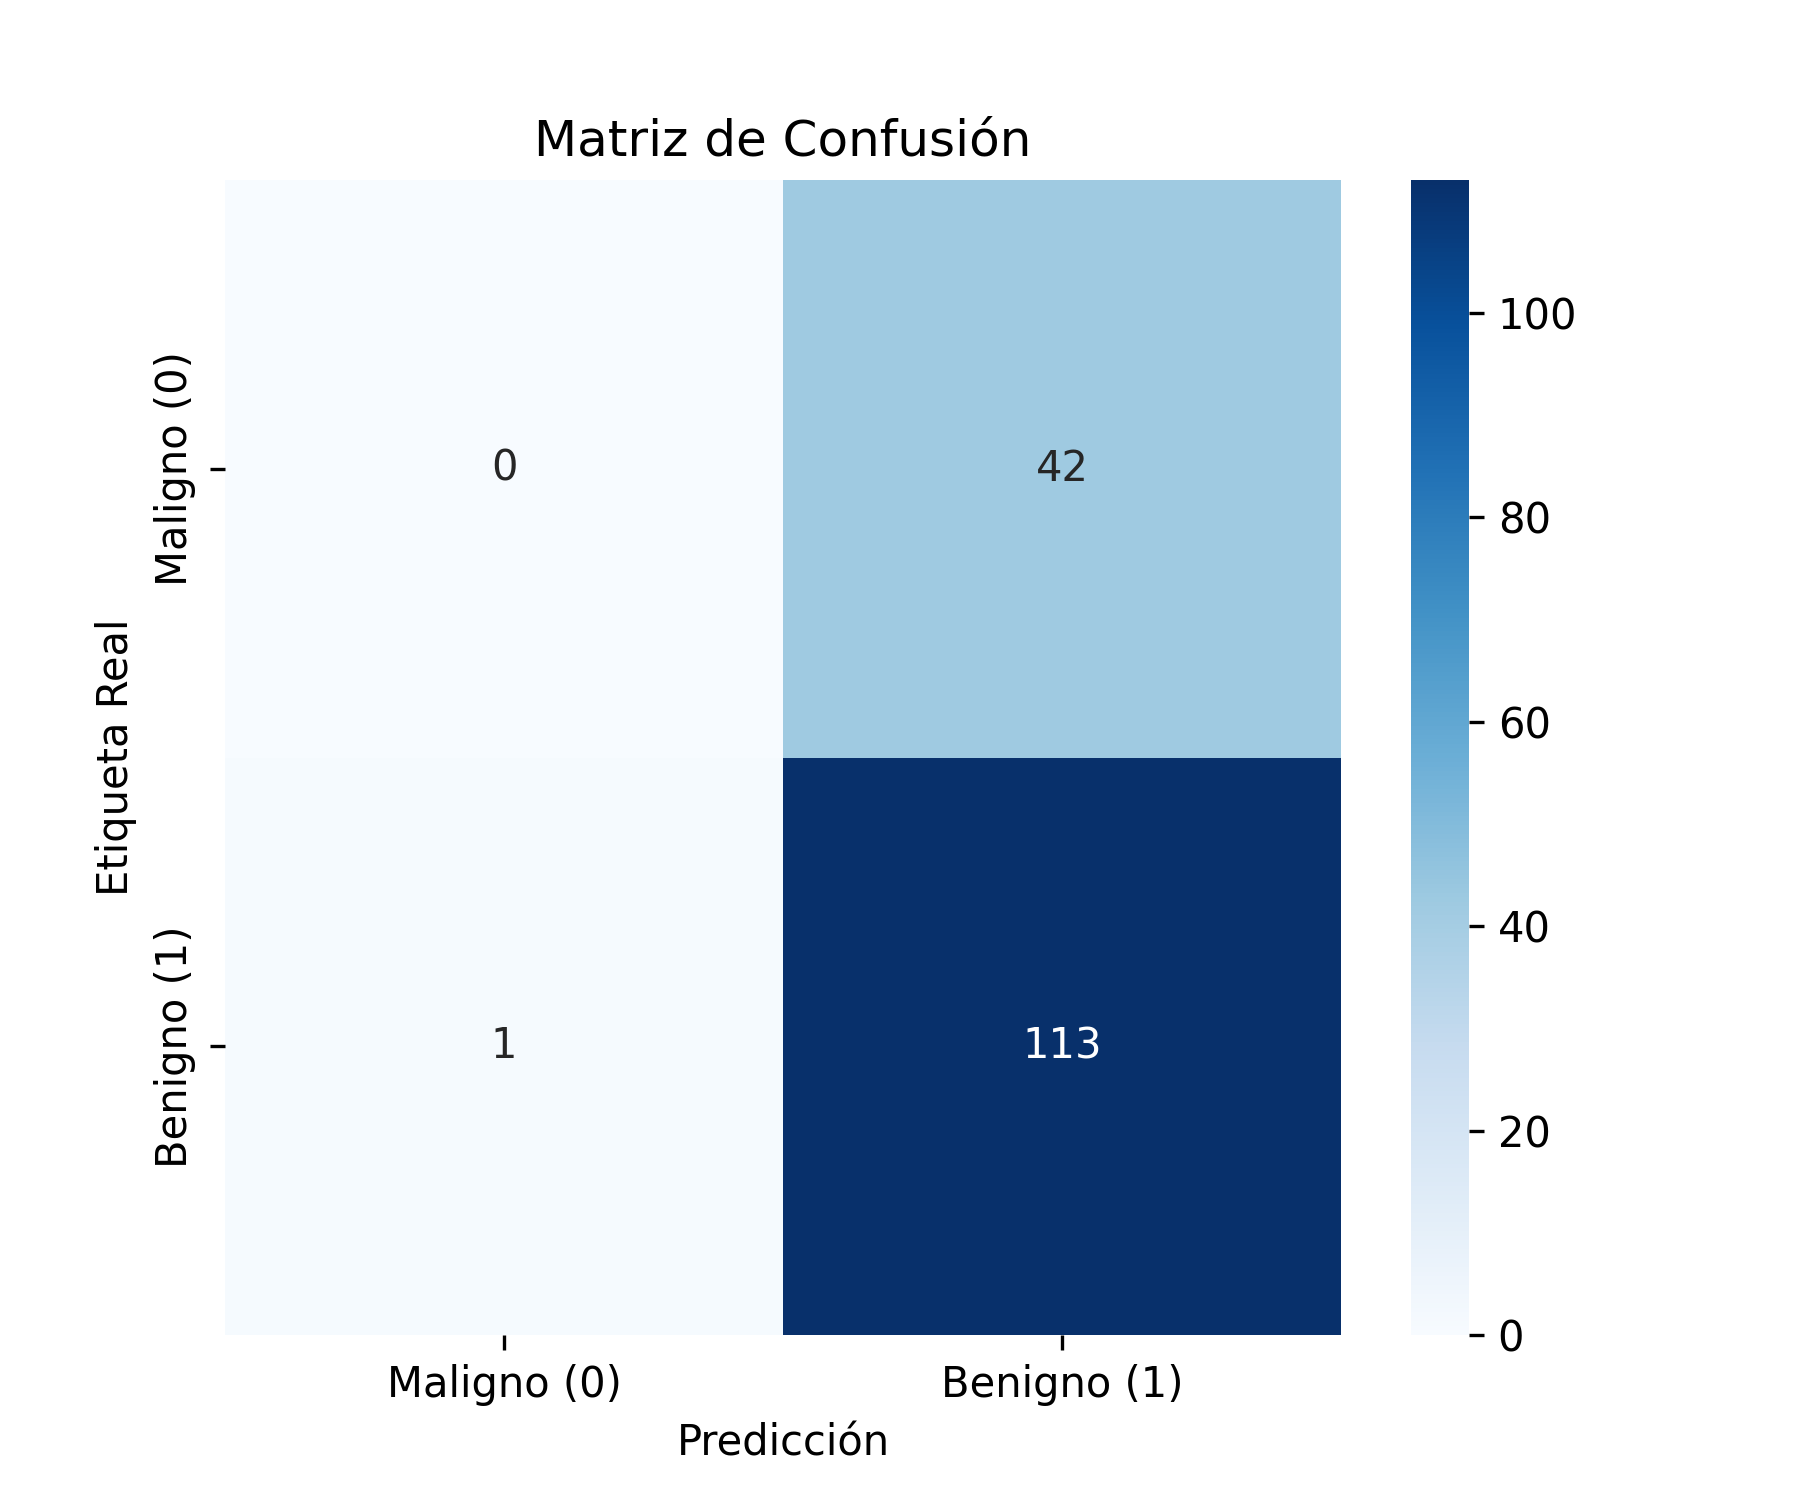
\includegraphics[width=0.62\textwidth]{confusion_matrix.png}
\caption{Matriz de confusion del modelo con mayor AUC: MobileNetV2 Baseline a $28\times28$ pixeles. Se observa el colapso hacia la clase mayoritaria (benigno/normal), caracteristico del desbalance de clases.}
\label{fig:confusion}
\end{figure}

\subsection{Analisis 1: Dominio del Baseline frente a la Complejidad Arquitectonica}

MobileNetV2 en resolucion nativa ($28\times28$) obtuvo el mejor AUC (0.7214), superando a arquitecturas considerablemente mas complejas. Este resultado es coherente con el principio del \textit{sesgo inductivo}: las capas convolucionales imponen suposiciones de localidad espacial y equivarianza a traslaciones que resultan apropiadas para detectar patrones relevantes en imagenes medicas de baja resolucion. La insercion de EfficientNetB0 con resolucion aumentada a $128\times128$ produjo un AUC inferior (0.6629): la expansion artificial mediante interpolacion bilineal no agrega informacion real, sino que introduce suavizado que dificulta la discriminacion. Este hallazgo sugiere que, en ausencia de datos de mayor resolucion real, el aumento de resolucion es contraproducente.

\subsection{Analisis 2: La Trampa del Recall y el Colapso de Clase}

Todos los modelos reportaron Accuracy = 0.7308 y Recall = 1.0 de manera identica. Esta combinacion es la signatura inequivoca del colapso hacia la clase mayoritaria: el modelo predice ``benigno'' para todas las muestras, obteniendo exactamente la proporcion de la clase mayoritaria en el conjunto de prueba. El Recall = 1.0 no indica un clasificador perfecto; indica que el modelo acierta en todos los casos benignos (la clase positiva mayoritaria) precisamente porque clasifica todo como benigno.

Este resultado subraya la conclusion central de \citet{yang2023medmnist}: en datasets biomedicos desbalanceados, el AUC-ROC es la unica metrica de primer orden. Un sistema con Accuracy = 0.73 y Recall = 1.0 puede parecer bueno, pero su especificidad es 0.0 (falla en el 100\% de los casos malignos), haciendo al modelo clínicamente inutil. La Figura~\ref{fig:confusion} confirma visualmente este patron.

\subsection{Analisis 3: Limitaciones del Vision Transformer en Datos Limitados}

El ViT en $128\times128$ supero a su variante en $28\times28$ en AUC (0.5512 vs. 0.4980), coherente con la arquitectura: los mecanismos de auto-atencion necesitan parches con suficiente contenido visual para aprender relaciones de largo alcance. Sin embargo, ambas variantes permanecieron por debajo de las CNN, con AUC cercano al azar (AUC = 0.5 corresponde a clasificacion aleatoria). Esto confirma el hallazgo teorico de \citet{dosovitskiy2021vit}: los Transformers sin pre-entrenamiento masivo no pueden competir con CNN en datasets de escala reducida. El ViT carece del sesgo inductivo de localidad espacial, confiando enteramente en los datos para descubrir estas estructuras. Con 546 muestras de entrenamiento, este proceso de descubrimiento es insuficiente.

\subsection{Analisis 4: Eficiencia Computacional}

El tiempo de entrenamiento es coherente con la complejidad de cada modelo. MobileNetV2 (0.27 min) ofrece el mejor balance rendimiento/costo, siendo ademas el de mayor AUC. El ViT en $128\times128$ es el mas costoso temporalmente (0.61 min) con el peor retorno en AUC entre los modelos no-triviales. En un contexto de despliegue clinico, la eficiencia de MobileNetV2 representa una ventaja adicional sobre el ViT de mayor resolucion.

% --- SECCION 5: CONCLUSIONES ---
\section{Conclusiones}

Este estudio comparativo demuestra que para el dataset BreastMNIST, con 546 muestras de entrenamiento y resolucion nativa de $28\times28$ pixeles, las arquitecturas convolucionales ligeras con sesgos inductivos espaciales ---particularmente MobileNetV2--- ofrecen la mejor relacion rendimiento/eficiencia. Los hallazgos principales son:

\begin{enumerate}
    \item \textbf{El sesgo inductivo de localidad} de las CNN constituye una ventaja decisiva en regimenes de datos pequenos y baja resolucion espacial.
    \item \textbf{El desbalance de clases} hace indispensable evaluar con AUC-ROC como metrica principal; el accuracy y el Recall aislados son metricas enganosas en diagnostico medico.
    \item \textbf{Los Vision Transformers sin pre-entrenamiento} a gran escala no son competitivos en datasets medicos de tamano reducido, confirmando los limites teoricos establecidos en la literatura \citep{dosovitskiy2021vit}.
    \item \textbf{La expansion artificial de resolucion} mediante interpolacion no aporta informacion real y puede degradar el rendimiento al introducir suavizado en los patrones diagnosticos.
\end{enumerate}

Como trabajo futuro se recomienda explorar: (a) pre-entrenamiento auto-supervisado (DINO, MAE) para adaptar ViT a datos medicos limitados; (b) tecnicas de balanceo de clases (\textit{class weighting}, SMOTE) para reducir el colapso hacia la clase mayoritaria; (c) uso de imagenes de ultrasonido de mayor resolucion real (sin interpolacion) para evaluar el potencial real de EfficientNet y ViT.

% --- SECCION 6: USO DE LLMS (REQUISITO OBLIGATORIO) ---
\section{Declaracion sobre el Uso de Modelos de Lenguaje}

Durante la estructuracion del pipeline de datos y la codificacion en TensorFlow, se utilizaron asistentes basados en IA (LLMs). Estas herramientas aceleraron la configuracion inicial de los entrenamientos y el diseno orientado a objetos del codigo. Sin embargo, presentaron una desventaja critica: alucinaron repetidamente al proponer dimensiones erroneas en los tensores al interactuar con la resolucion anomala de $28\times28$ pixeles de MedMNIST. Los modelos sugeridos fallaban internamente en sus capas de Pooling o en la division de parches para el ViT. Para corregir estos fallos, el equipo debio programar manualmente las capas \texttt{PatchExtract} y \texttt{PatchEmbedding}, adaptando el calculo de dimensiones al tamano exacto de la entrada.

% --- BIBLIOGRAFIA ---
\newpage
\bibliographystyle{apalike}
\begin{thebibliography}{9}

\bibitem[Al-Dhabyani et al., 2020]{aldhabyani2020busi}
Al-Dhabyani, W., Gomaa, M., Khaled, H., \& Fahmy, A. (2020).
\newblock Dataset of breast ultrasound images.
\newblock \textit{Data in Brief}, 28, 104863.
\newblock \url{https://doi.org/10.1016/j.dib.2019.104863}

\bibitem[Dosovitskiy et al., 2021]{dosovitskiy2021vit}
Dosovitskiy, A., Beyer, L., Kolesnikov, A., Weissenborn, D., Zhai, X., Unterthiner, T., Dehghani, M., Minderer, M., Heigold, G., Gelly, S., Uszkoreit, J., \& Houlsby, N. (2021).
\newblock An image is worth 16x16 words: Transformers for image recognition at scale.
\newblock In \textit{International Conference on Learning Representations (ICLR 2021)}.
\newblock arXiv:2010.11929.

\bibitem[Yang et al., 2023]{yang2023medmnist}
Yang, J., Shi, R., Wei, D., Liu, Z., Zhao, L., Ke, B., Pfister, H., \& Ni, B. (2023).
\newblock MedMNIST v2 -- A large-scale lightweight benchmark for 2D and 3D biomedical image classification.
\newblock \textit{Scientific Data}, 10(1), 41.
\newblock \url{https://doi.org/10.1038/s41597-022-01721-8}

\end{thebibliography}

\end{document}
